\documentclass{article}

% ---------------------------------------------------------------- %
% short package descriptions are copied from
% https://ctan.org/

% ---------------------------------------------------------------- %

% Accept different input encodings
\usepackage[utf8]{inputenc}

% Standard package for selecting font encodings
\usepackage[T1]{fontenc}

% ---------------------------------------------------------------- %

% Multilingual support for Plain TEX or LATEX
\usepackage[ngerman]{babel}

% ---------------------------------------------------------------- %

% Set all page margins to 1.5cm
\usepackage{fullpage}

% Margin adjustment and detection of odd/even pages
\usepackage{changepage}

% Flexible and complete interface to document dimensions
\usepackage{geometry}

% ---------------------------------------------------------------- %
% mathematics

\usepackage{amsmath}  % AMS mathematical facilities for LATEX
\usepackage{amssymb}
\usepackage{amsfonts} % TEX fonts from the American Mathematical Society
\usepackage{amsthm}   % Typesetting theorems (AMS style)

% Mathematical tools to use with amsmath
\usepackage{mathtools}

% Support for using RSFS fonts in maths
\usepackage{mathrsfs}

% Commands to produce dots in math that respect font size
\usepackage{mathdots}

% "Blackboard-style" cm fonts
\usepackage{bbm}

% Typeset in-line fractions in a "nice" way
\usepackage{nicefrac}

% Typeset quotient structures with LATEX
\usepackage{faktor}

% Vector arrows
\usepackage{esvect}

% St Mary Road symbols for theoretical computer science
\usepackage{stmaryrd}

% Three series of mathematical symbols
\usepackage{mathabx}

% ---------------------------------------------------------------- %
% algorithms

% Package for typesetting pseudocode
\usepackage{algpseudocode}

% Typeset source code listings using LATEX
\usepackage{listings}

% Reimplementation of and extensions to LATEX verbatim
\usepackage{verbatim}

% If necessary, please use the following 2 packages locally, but never both.
% This is because the algorithm environment gets defined in both packages, which leads to name conflicts.
% \usepackage{algorithm2e}
% \usepackage{algorithm}

% ---------------------------------------------------------------- %
% utilities

% A generic document command parser
\usepackage{xparse}

% Extended conditional commands
\usepackage{xifthen}

% e-TEX tools for LATEX
\usepackage{etoolbox}

% Define commands with suffixes
\usepackage{suffix}

% Extensive support for hypertext in LATEX
\usepackage{hyperref}

% Driver-independent color extensions for LATEX and pdfLATEX
\usepackage{xcolor}

% ---------------------------------------------------------------- %
% graphics

% -------------------------------- %

\usepackage{tikz}

% MISC
\usetikzlibrary{patterns}
\usetikzlibrary{decorations.markings}
\usetikzlibrary{positioning}
\usetikzlibrary{arrows}
\usetikzlibrary{arrows.meta}
\usetikzlibrary{overlay-beamer-styles}

% finite state machines
\usetikzlibrary{automata}

% turing machines
\usetikzlibrary{calc}
\usetikzlibrary{chains}
\usetikzlibrary{decorations.pathmorphing}

% -------------------------------- %

% Draw tree structures
\usepackage[noeepic]{qtree}

% Enhanced support for graphics
\usepackage{graphicx}

% Figures broken into subfigures
\usepackage{subfig}

% Improved interface for floating objects
\usepackage{float}

% Control float placement
\usepackage{placeins}

% Include PDF documents in LATEX
\usepackage{pdfpages}

% ---------------------------------------------------------------- %

% Control layout of itemize, enumerate, description
\usepackage[inline]{enumitem}

% Intermix single and multiple columns
\usepackage{multicol}
\setlength{\columnsep}{1cm}

% Coloured boxes, for LATEX examples and theorems, etc
\usepackage{tcolorbox}

% ---------------------------------------------------------------- %
% tables

% Tabulars with adjustable-width columns
\usepackage{tabularx}

% Tabular column heads and multilined cells
\usepackage{makecell}

% Publication quality tables in LATEX
\usepackage{booktabs}

% ---------------------------------------------------------------- %
% bibliography and quoting

% Sophisticated Bibliographies in LATEX
\usepackage[backend = biber, style = alphabetic]{biblatex}

% Context sensitive quotation facilities
\usepackage{csquotes}

% ---------------------------------------------------------------- %

% ---------------------------------------------------------------- %
% special letters

\newcommand{\N}{\mathbb N}
\newcommand{\Z}{\mathbb Z}
\newcommand{\Q}{\mathbb Q}
\newcommand{\R}{\mathbb R}
\newcommand{\C}{\mathbb C}
\newcommand{\K}{\mathbb K}
\newcommand{\T}{\mathbb T}
\newcommand{\E}{\mathbb E}
\newcommand{\V}{\mathbb V}
\renewcommand{\S}{\mathbb S}
\renewcommand{\P}{\mathbb P}
\newcommand{\1}{\mathbbm 1}
\newcommand{\G}{\mathbb G}

\newcommand{\iu}{\mathrm i}

% ---------------------------------------------------------------- %
% quantors

\newcommand{\Forall}        {\forall ~}
\newcommand{\Exists}        {\exists ~}
\newcommand{\nExists}       {\nexists ~}
\newcommand{\ExistsOnlyOne} {\exists! ~}
\newcommand{\nExistsOnlyOne}{\nexists! ~}
\newcommand{\ForAlmostAll}  {\forall^\infty ~}

% ---------------------------------------------------------------- %
% graphics boxed

\newcommand
{\includegraphicsboxed}
[2][0.75]
{
    \begin{center}
        \begin{tcolorbox}[standard jigsaw, opacityback = 0]

            \centering
            \includegraphics[width = #1 \textwidth]{#2}

        \end{tcolorbox}
    \end{center}
}

\newcommand
{\includegraphicsunboxed}
[2][0.75]
{
    \begin{center}
        \includegraphics[width = #1 \textwidth]{#2}
    \end{center}
}

\NewDocumentCommand
{\includegraphicsgraphicsboxed}
{ O{0.75} O{0.25} m m}
{
    \begin{center}
        \begin{tcolorbox}[standard jigsaw, opacityback = 0]

            \centering
            \includegraphics[width = #1 \textwidth]{#3} \\
            \vspace{#2 cm}
            \includegraphics[width = #1 \textwidth]{#4}

        \end{tcolorbox}
    \end{center}
}

\NewDocumentCommand
{\includegraphicsgraphicsunboxed}
{ O{0.75} O{0.25} m m}
{
    \begin{center}

        \centering
        \includegraphics[width = #1 \textwidth]{#3} \\
        \vspace{#2 cm}
        \includegraphics[width = #1 \textwidth]{#4}

    \end{center}
}

% ---------------------------------------------------------------- %
% braces

\newcommand{\pbraces}[1]{{\left  ( #1 \right  )}}
\newcommand{\bbraces}[1]{{\left  [ #1 \right  ]}}
\newcommand{\Bbraces}[1]{{\left \{ #1 \right \}}}
\newcommand{\vbraces}[1]{{\left  | #1 \right  |}}
\newcommand{\Vbraces}[1]{{\left \| #1 \right \|}}

\newcommand{\abraces}[1]{{\left \langle #1 \right \rangle}}

\newcommand{\floorbraces}[1]{{\left \lfloor #1 \right \rfloor}}
\newcommand{\ceilbraces} [1]{{\left \lceil  #1 \right \rceil }}

\newcommand{\dbbraces}    [1]{{\llbracket     #1 \rrbracket}}
\newcommand{\dpbraces}    [1]{{\llparenthesis #1 \rrparenthesis}}
\newcommand{\dfloorbraces}[1]{{\llfloor       #1 \rrfloor}}
\newcommand{\dceilbraces} [1]{{\llceil        #1 \rrceil}}

\newcommand{\dabraces}[1]{{\left \langle \left \langle #1 \right \rangle \right \rangle}}

\newcommand{\abs}  [1]{\vbraces{#1}}
\newcommand{\round}[1]{\bbraces{#1}}
\newcommand{\floor}[1]{\floorbraces{#1}}
\newcommand{\ceil} [1]{\ceilbraces{#1}}

% ---------------------------------------------------------------- %

% MISC

% metric spaces
\newcommand{\norm}[2][]{\Vbraces{#2}_{#1}}
\DeclareMathOperator{\metric}{d}
\DeclareMathOperator{\dist}  {dist}
\DeclareMathOperator{\diam}  {diam}

% O-notation
\newcommand{\landau}{{\scriptstyle \mathcal{O}}}
\newcommand{\Landau}{\mathcal{O}}

% ---------------------------------------------------------------- %

% math operators

% hyperbolic trigonometric function inverses
\DeclareMathOperator{\areasinh}{areasinh}
\DeclareMathOperator{\areacosh}{areacosh}
\DeclareMathOperator{\areatanh}{areatanh}

% special functions
\DeclareMathOperator{\id} {id}
\DeclareMathOperator{\sgn}{sgn}
\DeclareMathOperator{\Inv}{Inv}
\DeclareMathOperator{\erf}{erf}
\DeclareMathOperator{\pv} {pv}

% exponential function as power
\WithSuffix \newcommand \exp* [1]{\mathrm{e}^{#1}}

% operations on sets
\DeclareMathOperator{\meas}{meas}
\DeclareMathOperator{\card}{card}
\DeclareMathOperator{\Span}{span}
\DeclareMathOperator{\conv}{conv}
\DeclareMathOperator{\cof}{cof}
\DeclareMathOperator{\mean}{mean}
\DeclareMathOperator{\avg}{avg}
\DeclareMathOperator*{\argmax}{argmax}
\DeclareMathOperator*{\argsmax}{argsmax}

% number theory stuff
\DeclareMathOperator{\ggT}{ggT}
\DeclareMathOperator{\kgV}{kgV}
\DeclareMathOperator{\modulo}{mod}

% polynomial stuff
\DeclareMathOperator{\ord}{ord}
\DeclareMathOperator{\grad}{grad}

% function properties
\DeclareMathOperator{\ran}{ran}
\DeclareMathOperator{\supp}{supp}
\DeclareMathOperator{\graph}{graph}
\DeclareMathOperator{\dom}{dom}
\DeclareMathOperator{\Def}{def}
\DeclareMathOperator{\rg}{rg}

% matrix stuff
\DeclareMathOperator{\GL}{GL}
\DeclareMathOperator{\SL}{SL}
\DeclareMathOperator{\U}{U}
\DeclareMathOperator{\SU}{SU}
\DeclareMathOperator{\PSU}{PSU}
% \DeclareMathOperator{\O}{O}
% \DeclareMathOperator{\PO}{PO}
% \DeclareMathOperator{\PSO}{PSO}
\DeclareMathOperator{\diag}{diag}

% algebra stuff
\DeclareMathOperator{\At}{At}
\DeclareMathOperator{\Ob}{Ob}
\DeclareMathOperator{\Hom}{Hom}
\DeclareMathOperator{\End}{End}
\DeclareMathOperator{\Aut}{Aut}
\DeclareMathOperator{\Lin}{L}

% other function classes
\DeclareMathOperator{\Lip}{Lip}
\DeclareMathOperator{\Mod}{Mod}
\DeclareMathOperator{\Dil}{Dil}

% constants
\DeclareMathOperator{\NIL}{NIL}
\DeclareMathOperator{\eps}{eps}

% ---------------------------------------------------------------- %
% doubble & tripple powers

\newcommand
{\primeprime}
{{\prime \prime}}

\newcommand
{\primeprimeprime}
{{\prime \prime \prime}}

\newcommand
{\astast}
{{\ast \ast}}

\newcommand
{\astastast}
{{\ast \ast \ast}}

% ---------------------------------------------------------------- %
% derivatives

\NewDocumentCommand
{\derivative}
{ O{} O{} m m}
{
    \frac
    {\mathrm d^{#2} {#1}}
    {\mathrm d {#3}^{#2}}
}

\NewDocumentCommand
{\pderivative}
{ O{} O{} m m}
{
    \frac
    {\partial^{#2} {#1}}
    {\partial {#3}^{#2}}
}

\DeclareMathOperator{\Div}{div}
\DeclareMathOperator{\rot}{rot}

% ---------------------------------------------------------------- %
% integrals

\NewDocumentCommand
{\Int}
{ O{} O{} m m}
{\int_{#1}^{#2} #3 ~ \mathrm d #4}

\NewDocumentCommand
{\Iint}
{ O{} O{} m m m}
{\iint_{#1}^{#2} #3 ~ \mathrm d #4 ~ \mathrm d #5}

\NewDocumentCommand
{\Iiint}
{ O{} O{} m m m m}
{\iiint_{#1}^{#2} #3 ~ \mathrm d #4 ~ \mathrm d #5 ~ \mathrm d #6}

\NewDocumentCommand
{\Iiiint}
{ O{} O{} m m m m m}
{\iiiint_{#1}^{#2} #3 ~ \mathrm d #4 ~ \mathrm d #5 ~ \mathrm d #6 ~ \mathrm d #7}

\NewDocumentCommand
{\Idotsint}
{ O{} O{} m m m}
{\idotsint_{#1}^{#2} #3 ~ \mathrm d #4 \dots ~ \mathrm d #5}

\NewDocumentCommand
{\Oint}
{ O{} O{} m m}
{\oint_{#1}^{#2} #3 ~ \mathrm d #4}

% ---------------------------------------------------------------- %

% source:
% https://tex.stackexchange.com/questions/203257/tikz-chains-with-one-side-of-the-leftmost-node-thickbold

% #1 (optional): current state, e.g. $q_0$
% #2: cursor position, e.g. 1
% #3: number of displayed cells, e.g. 5
% #4: contents of cells, e.g. {$\triangleright$, $x_1$, \dots, $x_n$, \textvisiblespace}

\newcommand{\turingtape}[4][]
{
    \begin{tikzpicture}

        \tikzset{tape/.style={minimum size=.7cm, draw}}

        \begin{scope}[start chain=0 going right, node distance=0mm]
            \foreach \x [count=\i] in #4
            {
                \ifnum\i=#3 % if last node reset outer sep to 0pt
                    \node [on chain=0, tape, outer sep=0pt] (n\i) {\x};
                    \draw (n\i.north east) -- ++(.1,0) decorate [decoration={zigzag, segment length=.12cm, amplitude=.02cm}] {-- ($(n\i.south east)+(+.1,0)$)} -- (n\i.south east) -- cycle;
                \else
                    \node [on chain=0, tape] (n\i) {\x};
                \fi

                \ifnum\i=1 % if first node draw a thick line at the left
                    \draw [line width=.1cm] (n\i.north west) -- (n\i.south west);
                \fi
            }
 
            \node [right=.25cm of n#3] {$\cdots$};
            \node [tape, above left=.25cm and 1cm of n1] (q) {#1};
            \draw [>=latex, ->] (q) -| (n#2);

        \end{scope}

    \end{tikzpicture}
}

% ---------------------------------------------------------------- %

% ---------------------------------------------------------------- %
% amsthm-environments:

\theoremstyle{definition}

% numbered theorems
\newtheorem{theorem}             {Satz}[section]
\newtheorem{lemma}      [theorem]{Lemma}
\newtheorem{corollary}  [theorem]{Korollar}
\newtheorem{proposition}[theorem]{Proposition}
\newtheorem{remark}     [theorem]{Bemerkung}
\newtheorem{definition} [theorem]{Definition}
\newtheorem{example}    [theorem]{Beispiel}
\newtheorem{heuristics} [theorem]{Heuristik}

% unnumbered theorems
\newtheorem*{theorem*}    {Satz}
\newtheorem*{lemma*}      {Lemma}
\newtheorem*{corollary*}  {Korollar}
\newtheorem*{proposition*}{Proposition}
\newtheorem*{remark*}     {Bemerkung}
\newtheorem*{definition*} {Definition}
\newtheorem*{example*}    {Beispiel}
\newtheorem*{heuristics*} {Heuristik}

% ---------------------------------------------------------------- %
% exercise- and solution-environments:

% Please define this stuff in project ("main.tex"):
% \def \lastexercisenumber {...}

\newtheorem{exercise}{Aufgabe}
\setcounter{exercise}{\lastexercisenumber}

\newenvironment{solution}
{
  \begin{proof}[Lösung]
}{
  \end{proof}
}

% ---------------------------------------------------------------- %
% MISC translations for environment-names

\renewcommand{\proofname} {Beweis}
\renewcommand{\figurename}{Abbildung}
\renewcommand{\tablename} {Tabelle}

% ---------------------------------------------------------------- %

\newtheorem{inneralgebraUE}{UE}
\newenvironment{algebraUE}[1]
{
  \renewcommand \theinneralgebraUE{#1} \inneralgebraUE
}
{\endinneralgebraUE}


\parskip 0pt
\parindent 0pt

\title
{
  Algebra - Übung 11 \\
  \vspace{4pt}
  \normalsize
  \textit{12. UE am 23.06.2020}
}
\author
{
  Richard Weiss       \and
  Florian Schager     \and
  Christian Sallinger \and
  Fabian Zehetgruber  \and
  Paul Winkler        \and
  Christian Göth
}
\date{}

\begin{document}

\maketitle

\begin{algebraUE}{384}
Sei $R$ der Polynomring $(\Z/5\Z)[t]$, und sei $U \subseteq R$ der kleinste
Unterring mit $1$ von $R$, der das Polynom $t^5$ enthält. Geben Sie ein Polynom
$p(x) \in U[x]$ an, welches in $R$ die Nullstelle $t$ hat. (Wenn Ihnen das zu
leicht ist: Finden Sie so ein Polynom, welches in $U[x]$ irreduzibel ist.)
\end{algebraUE}

\begin{solution}
\begin{align*}
  U &= \left\{\sum_{k = 0}^na_kt^{5k}: n \in \N, a_k \in \Z/5\Z, k = 0,\dots,n\right\} \\
  p(x) &= x^5 - t^5.
\end{align*}
Über $R$ ist $t$ die einzige Nullstelle von $p(x)$. Polynomdivision liefert
\begin{align*}
  (x^5-t^5):(x-t) = x^4 + tx^3 + t^2x^2 + t^3x + t^4.
\end{align*}

Da jedes lineare Polynom
eine Nullstelle in $U$ besitzt, bleibt als einzige Möglichkeit zur Reduktion
in irreduzible Faktoren die Faktorisierung in ein Polynom $q(x)$ 2-ten und ein Polynom
$r(x)$ 3-ten Grades übrig (o.B.d.A. normiert).
Angenommen
\begin{align*}
  p(x) &= q(x)r(x) = (x^3 + bx^2 + cx + d)(x^2 + fx + g) \\
  &= x^5 + (f + b)x^4 + (g + bf + c)x^3 +(bg + cf + d)x^2 + (cg + df)x + dg.
\end{align*}

\end{solution}

\begin{algebraUE}{386}

  \begin{itemize}
      \item[1.] Sei $p \in \mathbb{P}, k, n \in \mathbb{N}, n \geq 1.$ Dann ist $\varphi: a \mapsto a^p$ ein Automorphismus von GF($p^n$).
      \item[2.] Die in der Automorphismengruppe Aut(GF($p^n$)) von $\varphi$ erzeugte Untergruppe besteht aus allen $\varphi^k: a \mapsto a^{p^k}$ mit $k \in \{0, ..., n-1\}.$
      \item[3.] Jeder Automorphismus $\varphi$ eines Körpers $K$ lässt seinen Primkörper $P$ punktweise fest.
      \item[4.] Jeder Automorphismus von GF($p^n$) ist von der Form $a \mapsto a^{p^k}.$
  \end{itemize}
\end{algebraUE}

\begin{solution}
  \begin{itemize}
      \item[1.] $\varphi$ ist ein Körperhomomorphismus wegen
      \begin{align}
          \varphi(a + b) = (a + b)^p = a^p + b^p = \varphi(a) + \varphi(b), \\
          \varphi(ab) = (ab)^p = a^p b^p = \varphi(a) \varphi(b), \\
          \varphi(0) = 0.
      \end{align}

  Die Injektivität gilt wegen
  \begin{align}
      \varphi(a) = \varphi(b) \Longleftrightarrow a^p = b^p \Longleftrightarrow (a-b)^p = 0 \Longleftrightarrow a - b = 0.
  \end{align}
  Weil GF($p^n$) eine endliche Menge ist, folgt aus Injektivität schon Surjektivität.

  \item[2.] Es gilt $\langle\varphi\rangle = \{\varphi^k~|~ 0 \leq k \leq \mathrm{ord}(\varphi)\}.$ Nach Proposition 6.3.3.2 (5) gibt es genau $n$ Automorphismen von GF($p^n$), es muss also $\mathrm{ord}(\varphi) < n$ gelten.

  \item[3.] $P$ wird als $\text{Ring}_1$ von der leeren Menge erzeugt. Da ein Automorphismus bereits durch seine Einschränkung auf ein Erzeugendensystem eindeutig bestimmt ist, kann es damit nur einen Automorphismus geben. Die Identität ist ein solcher und folglich auch der einzige.

  \item[4.] Wir zeigen noch, dass die Automorphismen $\varphi^k, k \in \{0, ..., n-1\}$ alle verschieden sind. Angenommen, es gäbe $i, j < n, i \neq j$ mit $a^{p^i} = a^{p^j}$ für alle $a.$ Die multiplikative Gruppe GF($p^n$)* hat ein erzeugendes Element $\alpha.$ Insbesondere gilt für dieses
  \begin{align}
      1 = \alpha^{p^j - p^i}
  \end{align}
  im Widerspruch zu $\mathrm{ord}(\alpha) = p^n - 1$. Es gibt also genau $n$ Frobeniusautomorphismen.

  Ein beliebiger Automorphismus $\psi$ ist eindeutig durch seinen Wert für $\alpha$ festgelegt. Sei $f$ das Minimalpolynom von $\alpha$ über $P.$ Nach Proposition 6.3.3.2 (4) kommen als Werte für $\alpha$ unter $\psi$ genau die $n$ verschiedenen Nullstellen von $f$ infrage \textbf{(warum kann keine Nullstelle doppelt vorkommen?)}. Es gibt also $n$ Automorphismen, genauso viele wie Frobeniusautomorphismen.

\end{solution}

\begin{exercise}

Hier könnte Ihre Werbung stehen!

\begin{itemize}
    \item[(a)] $F$ und $G$ seien (Wahrscheinlichkeits-) Verteilungsfunktionen, $d$ die Lévy-Prohorov-Metrik. Zeigen Sie für die verallgemeinerten Inversen

    \begin{equation*}
      d(F^{-1},G^{-1}) \leq d(F,G).
    \end{equation*}

    \item[(b)] Zeigen Sie: $F_n \longrightarrow F$ genau dann, wenn es auf einem geeigneten Wahrscheinlichkeitsraum Zufallsvariablen $X_n \sim F_n, X \sim F$ gibt mit $X_n \rightarrow X$ fast sicher (Darstellungssatz von Skorohod).
\end{itemize}

\end{exercise}

\begin{solution}

(a) Die verallgemeinerte Inverse wird definiert für $p \in (0, 1]$.

\begin{align*}
  F^{-1}(p) := \inf \Bbraces{x \in \R: p \leq F(x)}
\end{align*}

Wir benennen die folgenden Mengen.

\begin{align*}
  A  & := \Bbraces
  {
    \epsilon > 0:
    \Forall x \in \R:
    F(x - \epsilon) - \epsilon \leq
    G(x) \leq
    F(x + \epsilon) + \epsilon
  } \\
  B & := \Bbraces
  {
    \epsilon > 0:
    \Forall x \in \R:
    F^{-1}(x - \epsilon) - \epsilon \leq
    G^{-1}(x) \leq
    F^{-1}(x + \epsilon) + \epsilon
  }
\end{align*}

Für $\inf B \leq \inf A$, genügt es $A \subseteq B$ zu zeigen. Sei also $\epsilon \in A$, dann gilt $\epsilon > 0$ und $\Forall x \in \R:$

\begin{align*}
  F(x - \epsilon) - \epsilon \leq
  G(x) \leq
  F(x + \epsilon) + \epsilon.
\end{align*}

Wir wollen zeigen, dass

\begin{align*}
  F^{-1}(x - \epsilon) - \epsilon \leq
  G^{-1}(x) \leq
  F^{-1}(x + \epsilon) + \epsilon.
\end{align*}

Wir zeigen die erste Ungleichung; die zweite geht (wahrscheinlich) analog. Für die letzte Ungleichung beachte man $M \subseteq N$.

\begin{align*}
  \inf \Bbraces{y \in \R: x - \epsilon \leq F(y)} - \epsilon
  & = \inf \Bbraces{y - \epsilon \in \R: x - \epsilon \leq F(y)} \\
  & = \inf \Bbraces{z \in \R: x - \epsilon \leq F(z + \epsilon)} \\
  & = \inf \underbrace
      {
        \Bbraces{z \in \R: x \leq F(z + \epsilon) + \epsilon}
      }_{=: N} \\
  & \leq \inf \underbrace
      {
        \Bbraces{y \in \R: x \leq G(y)}
      }_{=: M}
\end{align*}

(b) Wir betrachten den Wahrscheinlichkeitsraum $(]0, 1[, \B(]0, 1[), \lambda)$ und bemerken, dass $F_n, F: \R \to [0, 1]$. Die verallgemeinerten Inversen $F_n^{-1}, F^{-1}$ sind monoton und somit messbar, also $X_n := F_n^{-1}, X := F^{-1}$ Zufallsvariablen. \\

$\Rightarrow$: Es ist zu zeigen, dass

\begin{align*}
  \P(X_n \xrightarrow{n \to \infty} X) = 1.
\end{align*}

Schwache Konvergenz ist bekanntlich äquivalent zur Konvergenz in der Lévy-Prohorov-Metrik.

\begin{align*}
  F_n \xrightarrow[\text{schwach}]{n \to \infty} F
  \Leftrightarrow
  d(F_n, F) \xrightarrow{n \to \infty} 0.
\end{align*}

Laut (a) wissen wir also bereits, dass

\begin{align*}
  d(X_n, X) =
  d(F_n^{-1}, F^{-1}) \leq
  d(F_n, F) \xrightarrow{n \to \infty} 0.
  \label{schwache_konvergenz}
\end{align*}

Eine weitere Äquivalenz zur schwach Konvergenz, erlaubt $\Forall \omega \in \mathcal{C}(X):$

\begin{align*}
  X_n(\omega) \xrightarrow{n \to \infty} X(\omega).
\end{align*}

Weil in jedem Intervall eine rationale Zahl ist und $|\Q| = \aleph_0$, gibt es nur abzählbar viele $F_n$- bzw. $F$-konstante Bereiche. $X_n, X$ haben genau dort ihre Sprungstellen, also ebenfalls nur abzählbar viele, also bilden sie eine $\lambda$-Nullmenge. Q.E.D. \\

$\Leftarrow$: $\lambda$ ist auf unserem Wahrscheinlichkeitsraum endlich, also folgt mit dem Satz von Egorov und Übung 11, Beispiel 6, dass

\begin{align*}
  X_n \xrightarrow[\fastsicher]{n \to \infty} X
  \Rightarrow
  X_n \xrightarrow[\text{in WSK}]{n \to \infty} X
  \Rightarrow
  F_n \xrightarrow[\text{schwach}]{n \to \infty} F.
\end{align*}

\end{solution}

% --------------------------------------------------------------------------------

\begin{exercise}[265]

Zeigen Sie (nicht formal) $A \cup B \subseteq \bigcup \bigcup (A \times B)$.
(Achtung, das ist im Allgemeinen falsch. Fügen Sie zuerst eine sinnvolle Annahme
über $A$ und $B$ hinzu, damit der Satz auch stimmt.)

\end{exercise}

% --------------------------------------------------------------------------------

\begin{solution}
$A,B$ müssen beide nichtleer sein.
\begin{align*}
  A \times B &= \{(a,b): a \in A, b \in B\} = \{\{\{a\},\{a,b\}\}: a \in A, b \in B\} \\
  \bigcup (A \times B) &= \{ \{a\}: a \in A\} \cup \{\{a,b\}: a \in A, b \in B\}\\
  \bigcup \bigcup (A \times B) &= \bigcup \pbraces{\{ \{a\}: a \in A\} \cup \{\{a,b\}: a \in A, b \in B\}} = A \cup \Bbraces{x : x \in A \lor x \in B}
  \supseteq A \cup B.
\end{align*}

\end{solution}

\begin{exercise}
  Ziel dieser Aufgabe sit die Konstruktion eines Differenzenverfahrens für krumme
  Ränder. Sie dazu $E =(x_ic y_j) \in \R^2 \in \Omega$ ein Gitterpunkt im Inneren
  von $\Omega$, sodass die Gitterpunkte links $(x_i -h, y_j)$ und unterhalb
  $(x_i,y_j -h)$ von $E$ im Gebiet $\Omega$ liegen aber die Gitterpunkte rechts
  $(x_i + h, y_j)$ und oberhalb $(x_i, y_j + h)$ von $E$ nicht mehr in $\Omega$ liegen.
  Konstruieren Sie analog zu Aufgabe $59$ einen $5$-Punkt Differenzenstern für
  $\delta u(E)$, welcher $E$, die in $\Omega$ liegenden Nachbarpunkte $(x_i -h, y_j)$
  und $(x_i, y_j -h)$ sowie die Randpunkte
  $(x_i + \delta_x h , y_j), (x_i, y_j + \delta_y h) \in \partial \Omega$ mit
  $\delta_x, \delta_y \in (0,1)$ verwendet (siehe Abb. $2$). Welche Ordnung kann man
  erreichen?

  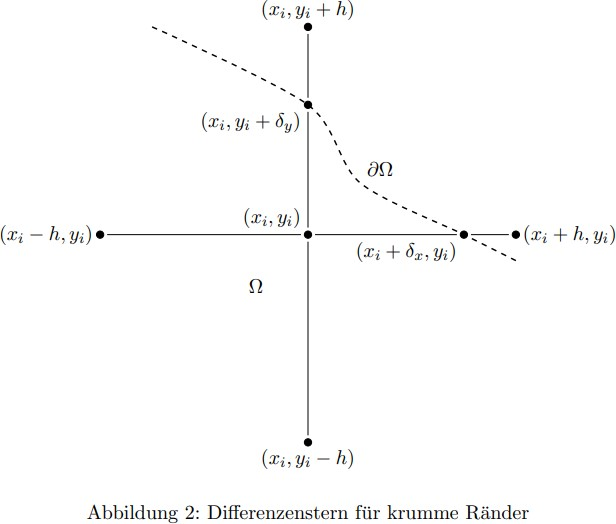
\includegraphics{Abbildung_2}
\end{exercise}

\begin{solution}
  Beweis.
\end{solution}

\begin{algebraUE}{397}
Sei $p \in \P$ eine Primzahl. Zeigen Sie, dass $GF(p^{\infty})$ überabzählbar viele
nichtisomorphe Unterkörper hat. \\
\textit{Anleitung:} Für jede (unendliche) Menge $A \subseteq \P$ sei $K_A$ Vereinigung
aller $GF(p^n)$, für die gilt, dass alle Primfaktoren von $n$ in $A$ liegen.
Schreiben Sie $K_A$ als aufsteigende Vereinigung $\bigcup_{j=1}^{\infty}U_j$
von Unterkörpern, um zu beweisen, dass $K_A$ ein Körper ist. Für $A \neq A^{\prime}$
zeigen Sie $K_A \ncong K_{A^\prime}$, indem Sie ein Polynom (wo liegen die
Koeffizienten dieses Polynoms?) finden, das zwar in $K_A$, aber nicht in $K_{A^{\prime}}$
eine Nullstelle hat, oder umgekehrt.
\end{algebraUE}

\begin{solution}

ToDo!

\end{solution}


\end{document}
